
\section{Overview of the proof strategy for $k \to \infty$}

The proof of Theorem~\ref{thm:mainktoinfty} follows the same strategy as outlined in Section~\ref{sec:proof_outline} and executed in Section~\ref{sec:proofs_fixed_k}. However, the fact that $k = k_n \to \infty$ as $n \to \infty$, introduces significant technical challenges, especially for $k_n$ close the the maximum scale $n^{\frac{1}{2\alpha + 1}}$. For example, the coupling between $\GPo$ and $\Gbox$ we use becomes less exact so that we can no longer use Lemma~\ref{lem:coupling_edges} to conclude that triangle counts in $\GPo$ and $\Gbox$ are asymptotically equivalent. Moreover, since we are ultimately interested in recovering the scaling of $c(k_n;G_n)$, which Theorem~\ref{thm:mainktoinfty} claims is $\gamma(k_n)$, we need to show that each step in the strategy outlined in Section~\ref{sec:proof_outline} only introduces error terms that are of smaller order, i.e. that are $\smallO{\gamma(k_n)}$. This will turn out to require a great deal of care in bounding all error terms we encounter.

In this section we explain the challenges with each step and give a detailed overview of the structure for the proof of Theorem~\ref{thm:mainktoinfty} using intermediate results for each of the steps. To this end we define the scaling function
\begin{equation}\label{eq:def_scaling_function}
	s(k) = \begin{cases}
		k^{-(4\alpha - 2)} &\mbox{if } \frac{1}{2} < \alpha < \frac{3}{4},\\
		\log(k) k^{-1} &\mbox{if } \alpha = \frac{3}{4},\\
		k^{-1} &\mbox{if } \alpha > \frac{3}{4},
	\end{cases}
\end{equation}
so that $\gamma(k) = \bigT{s(k)}$ as $k \to \infty$. We will end this section with the proof of Theorem~\ref{thm:mainktoinfty}, based on the intermediate results.

\begin{remark}[Diverging $k_n$]
Throughout the remainder of this paper, unless stated otherwise, $\{k_n\}_{n \ge 1}$ will always denote a sequence of integers satisfying $k_n \to \infty$ and $k_n = \smallO{n^{\frac{1}{2\alpha + 1}}}$, as $n \to \infty$.
\end{remark}

We start with introducing a slightly modified version of the local clustering function, which will be convenient for computations later,
\begin{equation}\label{eq:def_local_clustering_ast_general}
	c^\ast(k;G) = \frac{1}{\Exp{N_k}} \sum_{v \in V(G) \atop \text{deg}(v)=k} c(v).
\end{equation}
Notice that the only difference between $c(k;G)$ and $c^\ast(k;G)$ is that we replace $N_k$ by its expectation $\Exp{N_k}$. The advantage is that now, the only randomness is in the formation of triangles. In addition, note that since $\Exp{N_k} > 0$ a case distinction for $N_k$ is no longer needed for $c^\ast(k;G)$. It is however still relevant since we are eventually interested in $c(k;G)$. Following the notational convention, throughout the remainder of this paper we write $c^\ast(k; \GPo)$ and $c^\ast(k; \Gbox)$ to denote the modified local clustering function in $\GPo$ and $G_{\mathcal{P},n}(\alpha,\nu)$, respectively.

Figure~\ref{fig:overview_proof} shows a schematic overview of the proof of Theorem~\ref{thm:mainktoinfty} based on the different propositions described below, plus the sections in which theses propositions are proved. Observe that the order in which the intermediate results are proved is reversed with respect to the natural order of reasoning. This does not create any circular logic, since each intermediate result is independent of the others. We choose this order because results proved in the later stages are helpful to deal with error terms coming up in proofs at earlier stages and hence help streamline those proofs. Below briefly describe each of the intermediate steps leading up to the proof of Theorem~\ref{thm:mainktoinfty}. We start with an observation on the dependence between the degree of a point $p = (x,y)$ and its height $y$.

\subsection{Restricting the height for vertices with degree $k_n$}

In the proof of Proposition~\ref{prop:asymp} we used a result that allowed us to restrict integration over $y$ to the interval $[a(k)^-, a(k)^+]$, with
\[
	a(k)^\pm = 2\log\left(\frac{k \pm C \sqrt{k \log(k)}}{\xi} \vee 1\right).
\]
The reason for this was that the integrand included the function $\rho(y,k) = \Prob{\Po(\mu(y)) = k}$, where $\Po(\lambda)$ denotes a Poisson random variable with expectation $\lambda$ and Poisson random variables are well concentrated around their mean, i.e. around heights $y$ for which $\mu(y) \approx k$. Since $\mu(y) = \mu(\BallPo{y}) = \xi e^{y/2}$, this implies that integration with respect to $\rho(y,k)$ is concentrated around $y \approx 2\log(k/\xi)$. In the remainder of this paper we will often encounter integrands involving the function $\Prob{\Po(\mu_n(y)) = k}$, for some $\mu_n(y)$ which is asymptoticly equivalent to $\mu(y)$. In these case we also want to be able to restrict our integration around those heights $y$ for which $y \approx 2\log(k_n/\xi)$. Such results are established in Section~\ref{sec:concentration_argument}. Moreover, we prove that if $\mu_n$ corresponds to either $\Mu{\BallHyp{y}}$ or $\Mu{\BallPon{y}}$, then for a certain classs of functions $h$
\[
	\int_0^\infty h(y) \hat{\rho}_n(y,k_n) \alpha e^{-\alpha y} \dd y 
	= (1+\smallO{1}) \int_0^\infty h(y) \rho(y,k_n) \alpha e^{-\alpha y} \dd y,
\]
i.e. we may replace $\hat{\rho}_n(y,k_n)$ in the integrand with $\rho(y,k_n)$.

\begin{figure}[!t]
\centering

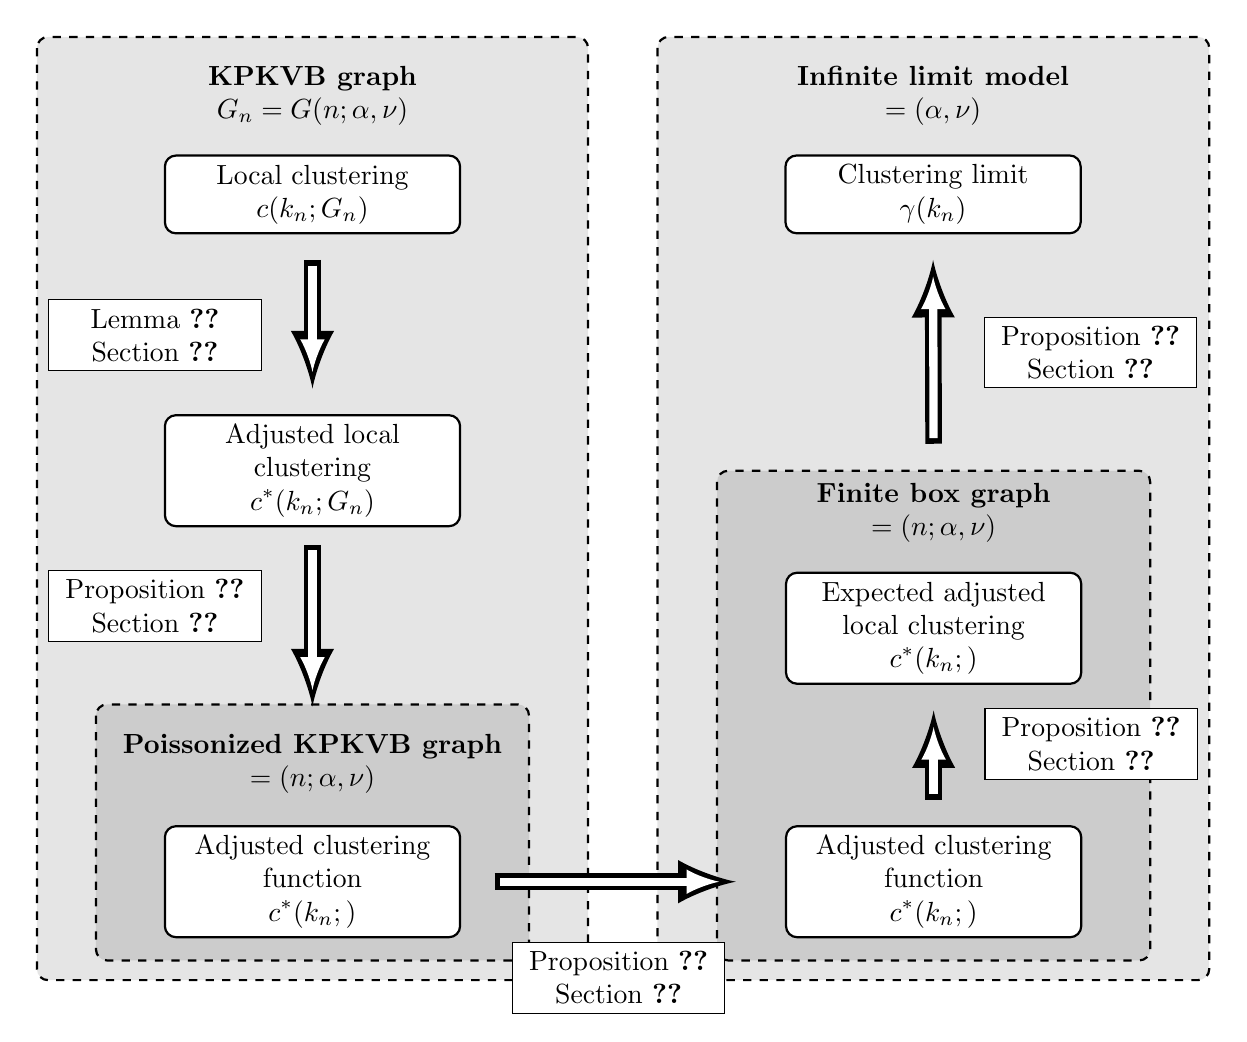
\begin{tikzpicture}

\pgfdeclarelayer{background}
\pgfdeclarelayer{foreground}
\pgfsetlayers{background,main,foreground}

\tikzstyle{block} = [draw, text centered, rounded corners, draw=black, thick, fill=white]
\tikzstyle{textblock} = [draw, text centered, draw=black, fill=white]

\tikzset{
  double arrow/.style args={#1 colored by #2 and #3}{
    -latex,line width=#1,#2, % first arrow
    postaction={draw,-latex,#3,line width=(#1)/2,
                shorten <=(#1)/3,shorten >=(#1)}, % second arrow
  }
}

\draw node (anchor) at (0,0) {};

%Hyperbolic graph: top left

\path (anchor)+(0,0) node (hyp_header) {\begin{minipage}[c]{10em}
	\begin{center}
		\textbf{KPKVB graph}\\
		$G_n = G(n; \alpha, \nu)$
	\end{center}
\end{minipage}};

\path (hyp_header.south)+(0,-0.75) node (c_hyp) [block] {\begin{minipage}[c]{10em}
	\begin{center}
	Local clustering\\
	$\displaystyle c(k_n;G_n)$
	\end{center}
\end{minipage}};






%Adjusted local clustering: middle left

\path (c_hyp.south)+(0,-3) node (c_ast_hyp) [block] {\begin{minipage}[c]{10em}
	\begin{center}
	Adjusted local clustering\\
	$\displaystyle c^\ast(k_n;G_n)$
	\end{center}
\end{minipage}};

\path (c_ast_hyp.north)+(-2,1) node (hyp_text) [textblock] {\begin{minipage}[c]{7em}
	\begin{center}
		Lemma \ref{lem:clustering_ast_H}\\
		Section~\ref{ssec:coupling_H_HP}
	\end{center}
\end{minipage}};

%Poisson Hyperbolic graph: middle left

%\path (c_hyp.south)+(0,-6) node (c_pois_hyp) [block] {\begin{minipage}[c]{12em}
%	\begin{center}
%	Local clustering\\
%	$\displaystyle c_{\widetilde{\H},n}(k_n)$
%	\end{center}
%\end{minipage}};



\path (c_ast_hyp.south)+(0,-3) node (pois_hyp_header) {\begin{minipage}[c]{14em}
	\begin{center}
		\textbf{Poissonized KPKVB graph}\\
		$\GPo = \GPo(n;\alpha,\nu)$
	\end{center}
\end{minipage}};

\path (pois_hyp_header.north)+(-2,1.5) node (pois_hyp_text) [textblock] {\begin{minipage}[c]{7em}
	\begin{center}
		Proposition \ref{prop:clustering_ast_H_Pois}\\
		Section~\ref{ssec:coupling_H_HP}
	\end{center}
\end{minipage}};





%Poisson Hyperbolic graph: bottom left

\path (pois_hyp_header.south)+(0,-1) node (c_ast_pois_hyp) [block] {\begin{minipage}[c]{10em}
	\begin{center}
	Adjusted clustering function\\
	$\displaystyle c^\ast(k_n; \GPo)$
	\end{center}
\end{minipage}};



%Infinite limit model: top right



\path (hyp_header.east)+(6,0) node (pois_header) {\begin{minipage}[c]{10em}
	\begin{center}
		\textbf{Infinite limit model}\\
		$\Ginf= \Ginf(\alpha, \nu)$
	\end{center}
\end{minipage}};

\path (pois_header)+(0,-1.25) node (c_infty) [block] {\begin{minipage}[c]{10em}
	\begin{center}
	Clustering limit\\
	$\displaystyle \gamma(k_n)$
	\end{center}
\end{minipage}};

\path (c_infty.south)+(2,-1.5) node (exp_c_pois_text) [textblock] {\begin{minipage}[c]{7em}
	\begin{center}
		Proposition \ref{prop:convergence_average_clustering_P_n}\\
		Section \ref{sec:clustering_Pn_to_P}
	\end{center}
\end{minipage}};




%Finite box model: bottom right

\path (c_ast_pois_hyp.east)+(6,0) node (c_ast_pois_n) [block] {\begin{minipage}[c]{10em}
	\begin{center}
	Adjusted clustering function\\
	$\displaystyle c^\ast(k_n; \Gbox)$
	\end{center}
\end{minipage}};

\path (c_ast_pois_n.south)+(-4,-0.5) node (c_ast_pois_n_text) [textblock] {\begin{minipage}[c]{7em}
	\begin{center}
		Proposition \ref{prop:couling_c_H_P}\\
		Section \ref{ssec:coupling_HP_ast_P}
	\end{center}
\end{minipage}};

\path (c_ast_pois_n.north)+(0,2.5) node (exp_c_pois_n) [block] {\begin{minipage}[c]{10em}
	\begin{center}
	Expected adjusted local clustering\\
	$\displaystyle \Exp{c^\ast(k_n; \Gbox)}$
	\end{center}
\end{minipage}};

\path (exp_c_pois_n.south)+(2,-0.75) node (exp_c_pois_n_text) [textblock] {\begin{minipage}[c]{7em}
	\begin{center}
		Proposition \ref{prop:concentration_local_clustering_P_n}\\
		Section \ref{sec:concentration_c_P_n}
	\end{center}
\end{minipage}};

\path (exp_c_pois_n.north)+(0,0.75) node (pois_n_header) {\begin{minipage}[c]{13em}
	\begin{center}
		\textbf{Finite box graph}\\
		$\Gbox = \Gbox(n; \alpha, \nu)$
	\end{center}
\end{minipage}};








%Arrows

\path (c_hyp.south)+(0,-0.2) node (arrow_1l) {};
\path (c_ast_hyp.north)+(0,0.2) node (arrow_1r) {};

\draw [double arrow=6pt colored by black and white] (arrow_1l) -- (arrow_1r);

\path (c_ast_hyp.south)+(0,-0.1) node (arrow_2l) {};
\path (pois_hyp_header.north)+(0,0.1) node (arrow_2r) {};

\draw [double arrow=6pt colored by black and white] (arrow_2l) -- (arrow_2r);

\path (c_ast_pois_hyp.east)+(0.3,0) node (arrow_3l) {};
\path (c_ast_pois_n.west)+(-0.5,0) node (arrow_3r) {};

\draw [double arrow=6pt colored by black and white] (arrow_3l) -- (arrow_3r);

\path (c_ast_pois_n.north)+(0,0.2) node (arrow_4l) {};
\path (exp_c_pois_n.south)+(0,-0.2) node (arrow_4r) {};

\draw [double arrow=6pt colored by black and white] (arrow_4l) -- (arrow_4r);

\path (exp_c_pois_n.north)+(0,1.5) node (arrow_5l) {};
\path (c_infty.south)+(0,-0.2) node (arrow_5r) {};

\draw [double arrow=6pt colored by black and white] (arrow_5l) -- (arrow_5r);

\begin{pgfonlayer}{background}

\path (c_hyp)+(-3.5,2) node (hyp_a) {};
\path (c_ast_pois_hyp)+(3.5,-1.25) node (hyp_b) {};
\path[rounded corners, draw=black, dashed, thick, fill=black!10] (hyp_a) rectangle (hyp_b);

\path (pois_hyp_header)+(-2.75,0.75) node (pois_hyp_a) {};
\path (c_ast_pois_hyp)+(2.75,-1) node (pois_hyp_b) {};
\path[rounded corners, draw=black, dashed, thick, fill=black!20] (pois_hyp_a) rectangle (pois_hyp_b);

\path (c_infty)+(-3.5,2) node (pois_a) {};
\path (c_ast_pois_n)+(3.5,-1.25) node (pois_b) {};
\path[rounded corners, draw=black, dashed, thick, fill=black!10] (pois_a) rectangle (pois_b);

\path (exp_c_pois_n)+(-2.75,2) node (pois_n_a) {};
\path (c_ast_pois_n)+(2.75,-1) node (pois_n_b) {};
\path[rounded corners, draw=black, dashed, thick, fill=black!20] (pois_n_a) rectangle (pois_n_b);

\end{pgfonlayer}

\end{tikzpicture}

\caption{Overview of the proof strategy for Theorem \ref{thm:local_clustering_hyperbolic}. The left column denote the models in which the true hyperbolic balls are used while the right column contains the models that use an approximation of these. The most important part is the transition between these to setting which is accomplished by Proposition~\ref{prop:couling_c_H_P}.}
\label{fig:overview_proof}
\end{figure}


\subsection{Adjusted clustering and the Poissonized KPKVB model}\label{ssec:KPKVB_to_GPo_infinite_k}

Recall that the first step for the fixed $k$ case was to show that the transition from the KPKVB graph $G_n = G(n;\alpha,\nu)$ to the Poissonized version $\GPo$ did not influence clustering. Here we first make a transition from the local clustering function $c(k_n; G_n)$ to the adjusted version $c^\ast(k_n; G_n)$. The following lemma justifies working with this modified version. The proof uses a concentration result for $\N_{n}(k_n)$ and full details can be found in Section~\ref{ssec:coupling_H_HP}.

\begin{lemma}\label{lem:clustering_ast_H}
As $n \to \infty$,
\[
	\Exp{\left|c(k_n;G_n) - c^\ast(k_n;G_n)\right|} = \smallO{s(k_n)}.
\]
\end{lemma}

We then establish that the modified local clustering function for KPKVB graphs $G_n$ behaves similarly to that in the $\GPo$. The proof, found in Section~\ref{ssec:coupling_H_HP}, is based on a standard coupling between a Binomial Point Process and Poisson Point Process.

\begin{proposition}\label{prop:clustering_ast_H_Pois}
As $n \to \infty$,
\[
	\Exp{\left|c^\ast(k_n;G_n) - c^\ast(k_n; \GPo)\right|} = \smallO{s(k_n)}.
\]
\end{proposition}

\subsection{Coupling of local clustering between $\GPo$ and $\Gbox$}

The next step is to show that the modified clustering is preserved under the coupling described in Section~\ref{ssec:coupling_H_P}. The proof can be found in Section~\ref{ssec:coupling_HP_ast_P}. This step is one of the key technical challenges we face in proving Theorem~\ref{thm:mainktoinfty}. 

To understand why, recall that the degree $k$ of a node is related to its height $y$, roughly speaking, by $k \approx \xi e^{y/2}$. Therefore, when $k$ is fixed we have that the heights of nodes with that degree are also fixed, in particular $y < R/4$ for large enough $n$. In addition, the main contribution of triangles would also come from nodes with heights $y^\prime < R/4$. This allowed us to use Lemma~\ref{lem:coupling_edges} and conclude that the triangles present in the graph $\GPo$ where exactly those present in $\Gbox$ and therefore the local clustering function was the same in both models. When $k_n \to \infty$ this is no longer true in general. For instance, suppose $k_n = n^{\frac{1-\varepsilon}{2\alpha + 1}}$, for some small $0 < \varepsilon < 1$. Then the relation $k_n \approx \xi e^{y_n/2}$ implies that $y_n \approx \frac{2(1-\varepsilon)}{2\alpha + 1}\log(n) - 2\log(\xi)$. Since
$R/4 = \frac{1}{2}\log(n) - \frac{1}{2}\log(\nu)$ we get that $R/4 = \smallO{y_n}$ for all $\alpha > (3 - 4\varepsilon)/2$ and hence $y_n > R/4$ for large enough $n$, violating the conditions of Lemma~\ref{lem:coupling_edges}. However, by carefully analyzing the difference between the adjusted local clustering function in both models we can still make the same conclusion. This is summarized in the following proposition whose proof is found in Section~\ref{ssec:coupling_HP_ast_P}.

\begin{proposition}[Coupling result for adjusted clustering function]\label{prop:couling_c_H_P}
As $n \to \infty$,
\[
	\Exp{\left|c^\ast(k_n; \GPo) - c^\ast(k_n; \Gbox)\right|} = \smallO{s(k_n)}.
\]
\end{proposition}

\TM{ Maybe we could replace these three with a statement on $|c(k_n;G_n) - c^\ast(k_n; \Gbox)|$, at least at this point of the paper. This is only the high level description and that is all we need for the ``final proof".}\PvdH{I would vote for keeping them split, since this allows us to clearly point to the main technical challenge we have to overcome to obtain the final result.}

Together, the three results described so far imply that the difference between the clustering function for a KPKVB graph and the adjusted clustering function for the finite box graph $\Gbox$ converges to zero faster than the proposed scaling $\gamma(k_n)$ in Theorem~\ref{thm:mainktoinfty}. Hence, to prove this theorem it is enough to prove it for $c^\ast(k; \Gbox)$. 

\subsection{From the finite box to the infinite model}

To compute the limit of the adjusted clustering function $c^\ast(k; \Gbox)$ we first prove in Section~\ref{sec:concentration_c_P_n} that it is concentrated around its mean $\Exp{c^\ast(k_n; \Gbox)}$.

\TM{ ``concentration'' is a loaded term in probability. I am not sure this use of the word will not be counterintuitive to many. }\PvdH{I am not sure. Concentration generally refers to how much a random variable deviates from its expectation. This is exactly what this proposition tells us. I would therefore vote for keeping this terminology, although I would have no problem with replacing it with an other term if someone has a good suggestion.}

\begin{proposition}[Concentration for adjusted clustering function in $\Gbox$]\label{prop:concentration_local_clustering_P_n}
As $n \to \infty$,
\[
	\Exp{\left|c^\ast(k_n; \Gbox) - \Exp{c^\ast(k_n; \Gbox)}\right|} = \smallO{s(k_n)}.
\]
\end{proposition}

This result represents another technical challenge we face when considering $k_n \to \infty$. For the proof, we first identify the specific range of heights that give the main contribution to the triangle count, showing that the triangles coming from nodes with heights outside this range is of smaller order. Then we prove a concentration result for the main term, by carefully analyzing the joint neighbourhoods of two nodes whose heights fall into the identified range. The full details are found in Section~\ref{sec:concentration_c_P_n}.

Assuming this concentration result, we are left to compute the limit of $\Exp{c^\ast(k_n; \Gbox)}$ as $n \to \infty$ and show that it is equivalent to $\gamma(k_n)$. To accomplish this we move to the infinite limit model $\Ginf$ and show that the difference between the expected value of $c^\ast(k;\Gbox)$ and $\gamma(k_n)$ goes to zero faster than the proposed scaling in Theorem \ref{thm:local_clustering_hyperbolic}.

\begin{proposition}[Transition to the infinite limit model]\label{prop:convergence_average_clustering_P_n}
As $n \to \infty$,
\[
	\left|\Exp{c^\ast(k_n; \Gbox)} - \gamma(k_n)\right| = \smallO{s(k_n)}.
\]
\end{proposition}

Recall that for the finite box model the left and right boundaries of $\Rcal_n$ where identified, so that graph $\Gbox$ contains some additional edge with respect to the induced subgraph of $\Ginf$ on $\Rcal_n$. The proof of Proposition~\ref{prop:convergence_average_clustering_P_n} therefore relies on analyzing the number of triangles coming from these additional edges and showing that their contribution to the clustering function are of negligible order, see Section~\ref{sec:clustering_Pn_to_P}. 

\begin{remark}[Notations different graphs]
We will use the subscripts $n$, $\Po$, $\text{box}$ and $\infty$ to identify properties of, respectively, the KPKVB mode $G_n$, the Poisson version $\GPo$, the finite box model $\Gbox$ and the infinite model $\Ginf$. For example $N_{\Po}(k)$ denotes number of nodes with degree $k$ in $\GPo$ and $\rho_{\text{box}}(y,k) = \Prob{\Po(\mu(\BallPo{y})) = k}$, i.e. the degree distribution in $\Gbox$ for a point $p = (x,y)$.
\end{remark}

\subsection{Proof of the main results}\label{ssec:proof_main_result_diverging_k}

We are now ready to prove Theorem~\ref{thm:mainktoinfty}, using the results stated in the previous sections.

\begin{proof}[Proof of Theorem~\ref{thm:mainktoinfty}]
Note that the second of the theorem follows immediately from the first.

To prove the first statement, we rewrite $c(k_n; G_n)$ as
\begin{align*}
    c(k_n;G_n)-\gamma(k_n) &= \left(c(k_n;G_n)-c^\ast(k_n;G_n)\right)
    	+ \left(c^\ast(k_n;G_n)-c^\ast(k_n; \GPo)\right)\\
    &\hspace{10pt}+ \left(c^\ast(k_n; \GPo)-c^\ast(k_n; \Gbox)\right)
    	+ \left(c^\ast(k_n; \Gbox)-\E c^\ast(k_n; \Gbox)\right)\\
    &\hspace{10pt}+ \E c^\ast(k_n; \Gbox)-\gamma(k_n)
\end{align*}
Then, we take absolute values and apply the triangle inequality. By monotonicity of expectation, we can apply it to both sides and obtain
\begin{align*}
    \Exp{\left|c(k_n;G_n)-\gamma(k_n)\right|} 
    &\le \Exp{\left|c(k_n;G_n)-c^\ast(k_n;G_n)\right|}
    	+\Exp{\left|c^\ast(k_n;G_n)-c^\ast(k_n; \GPo)\right|}\\
    &\hspace{10pt}+ \Exp{\left|c^\ast(k_n; \GPo)-c^\ast(k_n; \Gbox)\right|} 
    	+ \Exp{\left|c^\ast(k_n; \Gbox)-\E c^\ast(k_n; \Gbox)\right|}\\
    &+ \left|\Exp{c^\ast(k_n; \Gbox)}-\gamma(k_n)\right|
\end{align*}
At this point, the lemmas and propositions presented above in this section can be applied in order to show that all summands are $\smallO{\gamma(k_n)}$: Lemma~\ref{lem:clustering_ast_H} for the transition to the modified clustering function in the first term, Proposition~\ref{prop:clustering_ast_H_Pois} for the Poissonization in the second term, Proposition~\ref{prop:couling_c_H_P} for the coupling between the Poissonized KPKVB and the finite box model in the third term, Proposition~\ref{prop:concentration_local_clustering_P_n} for the concentration in the fourth term and finally Proposition~\ref{prop:convergence_average_clustering_P_n} for the transition to the infinite limit model. 

All of this together yields that:
\begin{align*}
    \Exp{\left|c(k_n;G_n)-\gamma(k_n)\right|} = \smallO{s(k_n)} = \smallO{\gamma(k_n)},
\end{align*}
which establishes the first statement of the theorem and finishes the proof.  
\end{proof}

